%%%%%%%%%%%%%%%%%%%%%%%%%%%%%%%%%%%%%%%%%%%%%%%%%%%%%%%%%%%%%%%%%%%%%%%%%%%%%%%%
%2345678901234567890123456789012345678901234567890123456789012345678901234567890
%        1         2         3         4         5         6         7         8

\documentclass[letterpaper, 10 pt, conference]{ieeeconf}  % Comment this line out if you need a4paper
\usepackage{amsmath, xparse}
\usepackage{amstext}
\usepackage{amsfonts}
\usepackage{float}
\usepackage{graphicx}

%\documentclass[a4paper, 10pt, conference]{ieeeconf}      % Use this line for a4 paper

\IEEEoverridecommandlockouts                              % This command is only needed if
                                                          % you want to use the \thanks command

\overrideIEEEmargins                                      % Needed to meet printer requirements.

%In case you encounter the following error:
%Error 1010 The PDF file may be corrupt (unable to open PDF file) OR
%Error 1000 An error occurred while parsing a contents stream. Unable to analyze the PDF file.
%This is a known problem with pdfLaTeX conversion filter. The file cannot be opened with acrobat reader
%Please use one of the alternatives below to circumvent this error by uncommenting one or the other
%\pdfobjcompresslevel=0
%\pdfminorversion=4

% See the \addtolength command later in the file to balance the column lengths
% on the last page of the document

% The following packages can be found on http:\\www.ctan.org
%\usepackage{graphics} % for pdf, bitmapped graphics files
%\usepackage{epsfig} % for postscript graphics files
%\usepackage{mathptmx} % assumes new font selection scheme installed
%\usepackage{times} % assumes new font selection scheme installed
%\usepackage{amsmath} % assumes amsmath package installed
%\usepackage{amssymb}  % assumes amsmath package installed

\title{\LARGE \bf
Homework 2 Report
}


\author{Arrian Chi% <-this % stops a space
}


\begin{document}

\onecolumn


\maketitle
\thispagestyle{empty}
\pagestyle{empty}


%%%%%%%%%%%%%%%%%%%%%%%%%%%%%%%%%%%%%%%%%%%%%%%%%%%%%%%%%%%%%%%%%%%%%%%%%%%%%%%%

\begin{abstract}

In this homework, I reviewed the discrete elastic rod algorithm and the various preliminaries that lead to its derivation, with a focus on the computation of twist. 

\end{abstract}
\section{Chapter 6: Discrete Twist}
The following 3 questions involve the computation of twist for an arbitrary discrete rod. The first 2 questions involve the computation of a rod with $ N = 4 $ nodes at:
\[ \mathbf{x}_1 = \begin{bmatrix} 0.00 & 0.00 & 0.00 \end{bmatrix} \quad \]
\[ \mathbf{x}_2 = \begin{bmatrix} 0.50 & 0.00 & 0.00 \end{bmatrix} \quad \]
\[ \mathbf{x}_3 = \begin{bmatrix} 0.75 & 0.25 & 0.00 \end{bmatrix} \quad \]
\[ \mathbf{x}_4 = \begin{bmatrix} 0.75 & 0.50 & 0.25 \end{bmatrix} \quad \]


The rod has an adapted material frame and the first material directors \( \mathbf{m}_k^1 \) (with \( k = 1, \ldots, N-1 \)) are:


\[\mathbf{m}_1^1 = \begin{bmatrix} 0.00 & 0.00 & 1.00 \end{bmatrix} \quad \]
\[\mathbf{m}_2^1 = \begin{bmatrix} 0.00 & 0.00 & 1.00 \end{bmatrix} \quad \]
\[\mathbf{m}_3^1 = \begin{bmatrix} 0.00 & -\frac{1}{\sqrt{2}} & \frac{1}{\sqrt{2}} \end{bmatrix} \quad \]


\subsection*{Q1: Compute the discrete integrated twist of this rod.}
After initializing the node positions and material directors, we can compute the edge vectors to compute tangent vectors of each edge of the rod. This will be used in calculating the twist, where we parallel transport the material frame of the $(k -1)$-th edge to the $k$-th edge. The twist at the $k$-th edge is the signed angle of the vector we just obtained to the corresponding material frame director about the current tangent vector. With this method, we get the following twist values for the rod:
\[ \tau_2 = 0 \ \text{at} \ \mathbf{x_2}\]
\[\tau_3 = 0.34\ \text{at} \ \mathbf{x_3} \]

\subsection*{Q2: Construct the space-parallel frame for the previous rod. Start with $u^1_1 = [0, 0, 1]$ at the first edge and use parallel transport to compute the 3 directors at subsequent edges. Evaluate the angle $ \nu ^ k (k = 1, \dots , N - 1)$ at each edge. Compute the twist. }

We have now learned about the space-parallel reference frame and how to use it in computing twist. Like before, we compute the tangent vectors over the entire rod. We then compute the directors of the space-parallel reference frame of each edge by parallel transporting the director of the previous edge to the current edge. The twist can finally be calculated like before, by computing the signed angle between a space-parallel reference frame director and its corresponding material frame director about the current tangent vector at k. The twist values for the rod are the same as before:
\[ \tau_2 = 0 \ \text{at} \ \mathbf{x_2}\]
\[\tau_3 = 0.34\ \text{at} \ \mathbf{x_3} \]

\subsection*{Q3: Given the node positions and twist angles at $t = 0, 0.05, \& 0.10$, compute the integrated discrete twist. Show your work. }

We finally learned about the time-parallel reference frame and its use case in computing twist over time. Here we are given the following DOFs at $t = 0, 0.05, \& 0.10$ in the form $\mathbf{x_{k-1}}, \theta_{k-1}, \mathbf{x_k}, \theta_k, \mathbf{x_{k+1}}, \theta_{k+1}, \dots$:
The given DOFs at different time steps are as follows:
At \( t = 0 \):
\[ q_0 = \begin{matrix}
\Bigl[2.000e-02 & 0.000e+00 & 0.000e+00 & 0.000e+00 & 6.306e-03  \\
1.898e-02 & 0.000e+00 & 0.000e+00 & -1.602e-02 & 1.197e-02  \\ 
0.000e+00 & 0.000e+00 & -1.641e-02 & -1.143e-02 & 0.000e+00 \\
0.000e+00 & 5.673e-03 & -1.918e-02 & 0.000e+00\Bigr]
\end{matrix} \]

At \( t = 0.05 \):
\[ q_1 = \begin{matrix}
\Bigl[ 2.000e-02 & 0.000e+00 & 0.000e+00 & 0.000e+00 & 6.306e-03 \\
1.898e-02 & 0.000e+00 & -2.006e-01 & -1.463e-02 & 1.281e-02 \\
-8.462e-03 & 2.191e-01 & -1.441e-02 & -8.443e-03 & -1.827e-02 \\
4.726e-01 & 7.321e-03 & -1.712e-02 & -1.796e-02 \Bigr]
\end{matrix} \]

At \( t = 0.10 \):
\[ q_2 = \begin{matrix}
\Bigl[ 2.000e-02 & 0.000e+00 & 0.000e+00 & 0.000e+00 & 6.306e-03 \\
1.898e-02 & 0.000e+00 & -3.908e-01 & -1.119e-02 & 1.474e-02 \\
-1.497e-02 & 3.572e-01 & -9.813e-03 & 3.396e-04 & -3.337e-02 \\
9.616e-01 & 1.117e-02 & -9.421e-03 & -3.688e-02 \Bigr]
\end{matrix} \]


We use $u^1 = [-8.110e-01, -5.851e-01, -0.000e+00]$ for the first director of the space-parallel reference frame of the first edge. Now we compute the space parallel reference frame for t = 0 (after setting up the tangents from before). This is also the time-parallel reference frame for t = 0.
\[ 
\mathbf{a_1^1} = [-8.110e-01, -5.851e-01, -0.000e+00] \]
\[
\mathbf{a_1^2} = [ 2.996e-01, -9.541e-01,  0.000e+00] \]
\[
\mathbf{a_1^3} = [ 9.999e-01, -1.666e-02,  0.000e+00] \]
\[
\mathbf{a_1^4} = [ 3.311e-01,  9.436e-01,  0.000e+00] \]

The reference twist may be computed by taking the parallel transport of the first time-parallel reference director from the $(k - 1)$-th edge to the $k$-th edge across the rod and computing the signed angle from that vector to the k-th time-parallel reference director about the $k$-th tangent. We obtain the reference twist at t = 0 as:
\[
\Delta m_{2, \text{ref}} = 2.717e-05, \quad \Delta m_{3, \text{ref}} = 1.388e-17, \quad \Delta m_{4, \text{ref}} = 0.000e+00
\]

The integrated discrete twist can be computed by adding the $k$-th reference twist to the difference of the $k$-th and $(k - 1)$-th twist angles. The integrated discrete twist at t = 0 is:
\[
\tau_2 = 2.717e-05, \quad \tau_3 = 1.388e-17, \quad \tau_4 = 0.000e+00
\]

(I also computed the material frames from the twist angles, but for the sake of brevity, I will not include them here. Please refer to the code for the full computation.)

Following this, we calculate the time parallel reference frame by parallel transporting the previous time's reference frame director to the current time's reference frame (using the old and new tangents). Then, we repeat the previous process across the entire rod for the next time steps. 

At \( t = 0.05 \) the time-parallel reference directors are:
\[ 
\mathbf{a_1^1} = [-8.110e-01, -5.851e-01, -0.000e+00] \]
\[ 
\mathbf{a_1^2} = [ 2.838e-01, -9.589e-01, -3.077e-03] \]
\[ 
\mathbf{a_1^3} = [ 9.999e-01,  7.865e-03,  5.387e-03] \]
\[ 
\mathbf{a_1^4} = [ 3.708e-01,  9.287e-01,  2.807e-04] \]


We obtain the reference twist at t = 0.05 as:
\[ 
\Delta m_{2, \text{ref}} = -2.667e-01, \quad \Delta m_{3, \text{ref}} = -5.650e-01, \quad \Delta m_{4, \text{ref}} = -2.895e-01 
\]

And the integrated discrete twist at t = 0.05 is:
\[ 
\tau_2 = -4.673e-01, \quad \tau_3 = -1.453e-01, \quad \tau_4 = -3.602e-02 
\]

At \( t = 0.10 \), the time-parallel reference directors are:
\[ 
\mathbf{a_1^1} = [-8.110e-01, -5.851e-01, -0.000e+00] \]
\[ 
\mathbf{a_1^2} = [ 2.531e-01, -9.672e-01, -2.183e-02] \]
\[ 
\mathbf{a_1^3} = [ 9.982e-01,  4.799e-02,  3.714e-02] \]
\[ 
\mathbf{a_1^4} = [ 4.213e-01,  9.069e-01, -3.499e-03] \]

We obtain the reference twist at t = 0.10 as:
\[ 
\Delta m_{2, \text{ref}} = -5.050e-01, \quad \Delta m_{3, \text{ref}} = -1.028e+00, \quad \Delta m_{4, \text{ref}} = -6.649e-01 
\]

And the integrated discrete twist at t = 0.10 is:
\[ 
\tau_2 = -8.958e-01, \quad \tau_3 = -2.803e-01, \quad \tau_4 = -6.051e-02 
\]

\bigskip

\section{Chapter 7: Discrete Elastic Rods Algorithm} 

\subsection*{Q1: Describe your implementation of the DER algorithm.}

We first initialize our rod with the number of nodes, the time steps, and the necessary constants to calculate the initial conditions of the system (i.e. the masses, the positions, the weights, etc.). One important value we calculate is the undeformed reference lengths, which is used to calculate the voronoi lengths. This is important for our elastic energy calculations in the following equations.

Some preliminary calculations are done (i.e. the reference twist and the curvature) as well as picking the free DOFs we care about (we will omit the values in the free DOFs in our calculations). Finally, from here we can start our loop.

In the loop (from the 0th to however many time steps), we call an objective function that calculates the new positions, new velocities, and new time-parallel reference directors for the rod, given the current DOFs. The result is updated in the DOFs and we step in time at the end of the loop (making sure to save any data we need for plotting).

In the objective function, we implement the Newton-Raphson method to solve for the new DOFs. Given our initial guess and a set error, we loop until we reach a desired accuracy. In this loop, we compute the time-parallel reference directors and tangents to obtain the new reference twists and the material frames. We then calculate the elastic energy and forces involved in the stretching, bending, and twisting of the rod. This includes calculating the Jacobians required for the update step of the Newton-Raphson method. Finally, we accumulate all the forces and jacobians of the system together, impose our boundary conditions, and solve for the delta DOFs, which we add to the current DOFs to get the new DOFs. If we reach the desired accuracy (check our error against a tolerance), we return the new DOFs, otherwise, we repeat the process again.

\subsection*{Q1: Plot the z-coordinate of the last node with time.}

Fig. \ref{"fig:p2q1_last_node"} shows the plot of the z-coordinate of the last node with time. The last node is initially at the origin, but as time progresses, the position oscillates and dampens to a final position of approximately 0.04. Forthe simulation, I used a small $\Delta t = 0.01$ s and a large $N = 50$. 

\begin{figure}[!ht]
        \centering
        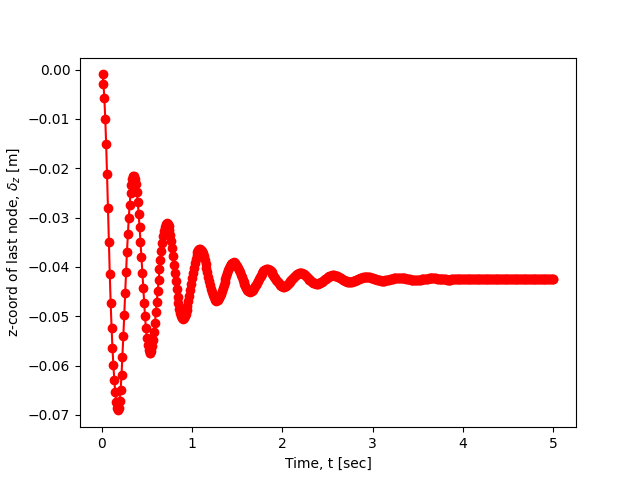
\includegraphics[width=0.7\textwidth,keepaspectratio]{last_node.png}
        \caption{Plot of the z-coordinate of the last node with time}
        \label{"fig:p2q1_last_node"}
\end{figure}




% \begin{figure}[!ht]
%         \centering
%         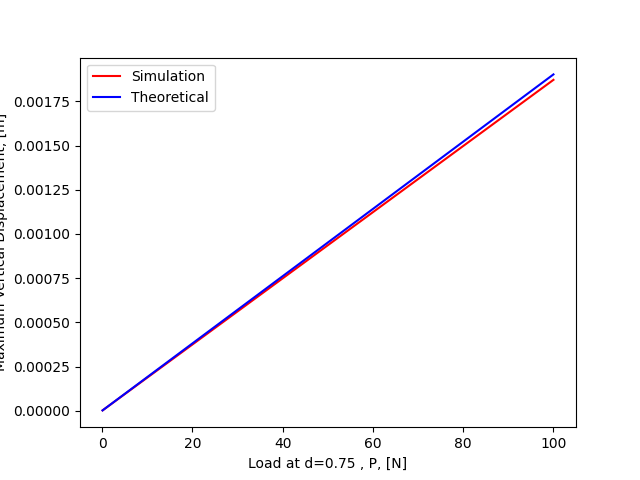
\includegraphics[width=0.45\textwidth,keepaspectratio]{p3_implicit_maxvert2xzoomed.png}
%         \caption{Plot of Maximum Vertical Displacement of the Beam v.s. the size of the point load (zoomed in again)}
%         \label{"fig:p3q2_benefit_zoomed2x"}
% \end{figure}

\addtolength{\textheight}{-12cm}   % This command serves to balance the column lengths
                                  % on the last page of the document manually. It shortens
                                  % the textheight of the last page by a suitable amount.
                                  % This command does not take effect until the next page
                                  % so it should come on the page before the last. Make
                                  % sure that you do not shorten the textheight too much.

%%%%%%%%%%%%%%%%%%%%%%%%%%%%%%%%%%%%%%%%%%%%%%%%%%%%%%%%%%%%%%%%%%%%%%%%%%%%%%%%



%%%%%%%%%%%%%%%%%%%%%%%%%%%%%%%%%%%%%%%%%%%%%%%%%%%%%%%%%%%%%%%%%%%%%%%%%%%%%%%%



\end{document}
